\documentclass[12pt]{report}
\usepackage[spanish, activeacute]{babel}
\usepackage[top=2.75cm,bottom=2.50cm,left=3.00cm,right=2.50cm]{geometry}
\usepackage[utf8]{inputenc}  
\usepackage{enumerate}
\usepackage{graphicx}



\begin{document}
	\setlength{\topmargin}{-0.5in}
	\pagestyle{empty}
	\begin{center}
		\textbf{
			\vspace{-0.7em}
			ESCUELA SUPERIOR POLITÉCNICA DEL LITORAL
		}
		\line(1,0){380}\\		
		\scriptsize{FACULTAD DE INGENIERÍA EN ELECTRICIDAD Y COMPUTACIÓN}
	\end{center}
	\begin{center}
		\vspace{2.5em}
		Lenguajes de Programación
		\\2012 | II Término
		\vspace{1.5em}
		\\Ana Arias - acarias@espol.edu.ec
		\vspace{4mm}
		\\Cesar Sanlucas - csan@espol.edu.ec
		\vspace{2em}
		\Huge{\textbf{\\Entrega tu Tarea!	\vspace{1em}}}
	\end{center}	


	\begingroup
		\large{
			\textbf{
				Descripción
				\newline
				\newline
			}
		}
	\endgroup

	%
	%Descripcion
	%
``Entrega tu Tarea! Es un divertido juego, con orientación educativa, puesto que de una forma entretenida, los niños podrán ejercitar su mente, sus habilidades matemáticas a través de un sano juego.
\newline
\newline
``Entrega tu Tarea tendrá como usuarios niños de jardin (4-5 años)  y de escuela (7-12 años). El objetivo es que el usuario vaya estructurando una tarea que consta de 3 partes: habilidad con la memoria, habilidades matemáticas, y habilidades visuales; otro objetivo es que el usuario pueda seguir correctamente las instrucciones que se le dan por medio de un audio.
\newline
\newline
Con una serie de audios e imágenes el usuario manejará facilmente este juego, y empezará a relacionar tareas diarias escolares con algo entretenido y práctico
\newline
\newline
Este juego está desarrollado en Python utilizando la librería Pygame, y como herramientas adicionales se utilizó Adobe Photoshop para la creación de imágenes y Audacity para la creación de audios.
	\newline
	\newline
	\newline
	\begingroup
		\large{
			\textbf{
				Funcionalidades
				\newline
				\newline
			}
		}
	\endgroup
	%
\newline
Entrega tu Tarea cuenta con muchas funcionalidades. Es un juego en el que con el paso de los niveles el usuario obtendrá cada vez mas habilidades.
\newline
\newline
La primera funcionalidad es la parte llamada "Memoriza", en esta parte el usuario tendrá que escuchar un audio con una secuencia de letras y números y despues ingresar correctamente dicha secuencia por teclado.
\newline
\newline
La segunda funcionalidad es la "Tarea matemática"  que consta de un ejercicio matemático conforme al nivel estudiantil y años que tiene el usuario, datos que se piden en el transcurso del juego.	
\newline
\newline	
Finalmente si el usuario ha respondido correctamente las tareas anteriores, tendrá que pasar por un divertido juego en el que tendrá que superar una serie de obtaculos para poder entregar su tarea exitosamente.
\newline
\newline
En el transcurso del juego, el usuario tendrá que seguir las instrucciones proporcionadas en audio.
\newline
\newline
El juego está hecho de forma que el usuario ingrese su nivel educativo(Jardín o escuela) y su edad; con estos datos, el programa escogerá que tipo de ejercicios matemáticos son los adecuados para la tarea.

\newpage

%--------------------------------------------------------------------------------------------------------------------
\begin{center}
	\begingroup
		
		\Huge{\textbf{\\Manual de Usuario	\vspace{1em}}}

	\endgroup
\end{center}
Inicio del juego. Escoja la opción que desee. Si desea jugar directamente, escoja por medio de las direccionales qué nivel educativo tiene y presione enter. Si desea conocer acerca de los creadores del programa, diríjase a la opción Creadores y presione enter


	\begin{center}
		\begingroup
			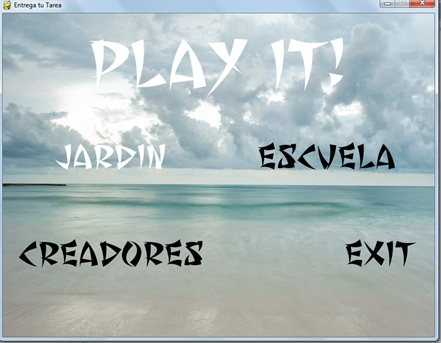
\includegraphics[width=0.6\textwidth]{imagenes_usuario/inicio.jpg}
		\endgroup
	\end{center}


%--------------------------------------------------------------------------------------------------------------------

Al escoger el nivel jardin o el nivel escuela, escuchará un audio con instrucciones. Esta es la tarea de "Memoria", memorice la secuencia e ingresela por teclado, al terminar de ingresar dicha secuencia presione la tecla F5.

	\begin{center}
		\begingroup
			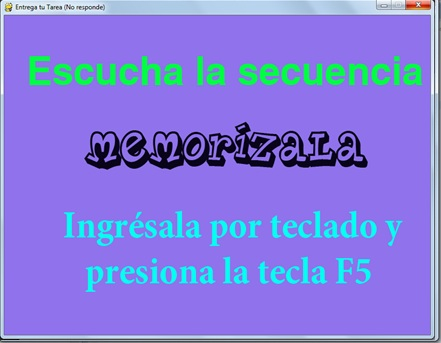
\includegraphics[width=0.6\textwidth]{imagenes_usuario/memoriza}
		\endgroup
	\end{center}

%--------------------------------------------------------------------------------------------------------------------

Inmediatamente saldrá un audio junto con una imagen que pedirán su edad, ingrésela por medio del teclado y cuando haya terminado presione la tecla F3

	\begin{center}
		\begingroup
			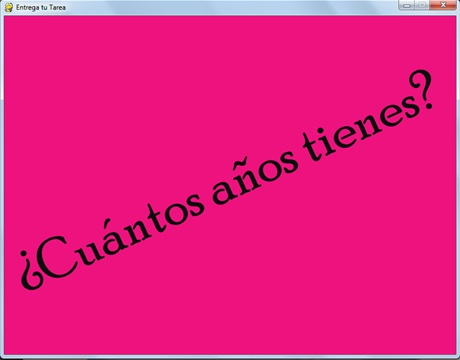
\includegraphics[width=0.6\textwidth]{imagenes_usuario/anios.jpg}
		\endgroup
	\end{center}


%--------------------------------------------------------------------------------------------------------------------

Después de haber ingresado su edad, pasará a la "Tarea Matemática", escuchará una serie de instrucciones y aparecerá una imagen con un ejercicio de matemáticas conforme al nivel educativo que ingresó al comienzo (Jardín o escuela) y de acuerdo a la edad que proporcionó anteriormente.
Resuelve el ejercicio, no hay límite de tiempo. Si se está seguro de la respuesta ingrésela por medio del teclado y presione la tecla F4.
Si la respuesta es incorrecta, escuchará un audio que le dirá que tiene una segunda oportunidad. El límite de equivocaciones es 3, si se equivoca mas de 3 veces, perderá.

	\begin{center}
		\begingroup
			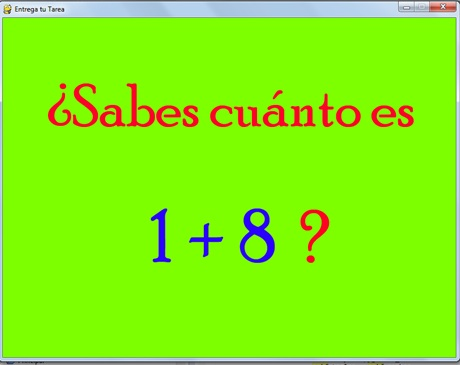
\includegraphics[width=0.6\textwidth]{imagenes_usuario/ejercicio.jpg}
		\endgroup
	\end{center}


%--------------------------------------------------------------------------------------------------------------------

Si se contestó correctamente, se pasará al juego, en el que se tendrá que pasar una serie de obstáculos para poder entregar su tarea exitosamente.
Escuchará las instrucciones respectivas del juego.
Muévase con las teclas direccionales (derecha: mover derecha, izquierda: mover izquierda, arriba: saltar) y dispare a las caritas felices con la tecla 1.

	\begin{center}
		\begingroup
			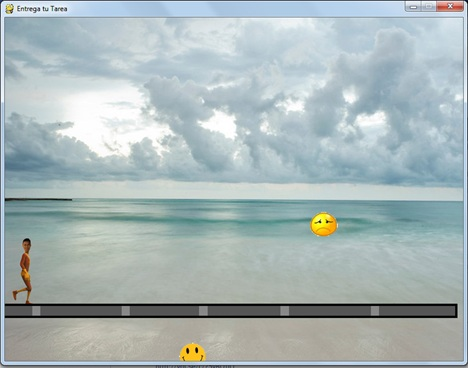
\includegraphics[width=0.6\textwidth]{imagenes_usuario/juego1.jpg}
		\endgroup
	\end{center}

%--------------------------------------------------------------------------------------------------------------------

Si se realizaron todas las tareas completamente, el usuario habrá ganado y entregado su tarea con exito!

	\begingroup
		\large{
			\textbf{
				\newline
				\newline
				\newline
				Experiencias con Python y Pygame
				\newline
				\newline
			}
		}
	\endgroup
	%

Cuando empezamos a estudiar Python, al iniciar este proyecto, nos encantó este lenguaje, nos pareció sencillo y totalmente completo; lo que nos pareció más interesante es la facilidad en la sintaxis del lenguaje, no es muy estricto como los otros lenguajes que dan mil errores por la falta de un punto y coma; sin embargo python se guía de manera excelente solo con identación; aunque nunca le habíamos puesto tanto interés en la identación, ahora lo hacemos  y lo haremos en cualquier lenguajes aunque no se trate de python.
\newline
\newline
Con respecto a Pygame, nos parecieron increíbles todas las funcionalidades que éste ofrece.
Al utilizar un ciclo while los juegos realizados en pygame, el manejar la actualizacion de los diferentes estados del juego (interfaz grafica) resultó un poco tedioso realizar el cambio de pantallas de nuestra aplicación.
\newline
\newline
El manejo de Sprites y GroupSprites disponibles en pygame nos resulto "mágico" debido a que esta clases nos provee mucha funcionalidades muy interesantes como por ejemplo para dibujar un objeto en pantalla ke herede de Sprite tan solo es necesario utilizar "el rectángulo e imagen del objeto" y el uso GroupSprites son un conjunto de Sprites y para dibujarlos hace uso de cada uno de los rectangulos e imagens de los Sprites que se encuentran en el grupo...
por esto darla apariencia de movimiento e interaccion del objeto tan solo fue necesario actualizar su posicion en pantalla (puntos x,y) y con estos actualizar el rectangulo del objeto.
\newline
\newline
Al comienzo del proyecto parecía un poco exagerado esto de hacer un “Video Juego” pero en el transcurso del proyecto esto se fue convirtiendo en una tarea más fácil y entretenida. Nos gustó mucho programar un Video Juego, espero mejorarlo con el tiempo.
En resumen fue una linda experiencia trabajar en este proyecto.


\end{document}


